% This must be in the first 5 lines to tell arXiv to use pdfLaTeX, which is strongly recommended.
\pdfoutput=1
% In particular, the hyperref package requires pdfLaTeX in order to break URLs across lines.

\documentclass[11pt]{article}

% Change "review" to "final" to generate the final (sometimes called camera-ready) version.
% Change to "preprint" to generate a non-anonymous version with page numbers.
\usepackage[final]{acl}

% Standard package includes
\usepackage{times}
\usepackage{latexsym}
\usepackage{tipa}
\usepackage{amsmath}
\usepackage{booktabs}
\usepackage{multirow}
\usepackage{graphicx} % For resizing
\usepackage{longtable}
% For proper rendering and hyphenation of words containing Latin characters (including in bib files)
\usepackage[T1]{fontenc}
\usepackage[utf8]{inputenc}
% For Vietnamese characters
% \usepackage[T5]{fontenc}
% See https://www.latex-project.org/help/documentation/encguide.pdf for other character sets



% This assumes your files are encoded as UTF8
\usepackage[utf8]{inputenc}

% This is not strictly necessary, and may be commented out,
% but it will improve the layout of the manuscript,
% and will typically save some space.
\usepackage{microtype}

% This is also not strictly necessary, and may be commented out.
% However, it will improve the aesthetics of text in
% the typewriter font.
\usepackage{inconsolata}

%Including images in your LaTeX document requires adding
%additional package(s)
\usepackage{graphicx}
\usepackage{tipa}
% If the title and author information does not fit in the area allocated, uncomment the following
%
%\setlength\titlebox{<dim>}
%
% and set <dim> to something 5cm or larger.

\title{ZIPA: A family of efficient models for multilingual phone recognition}

% Author information can be set in various styles:
% For several authors from the same institution:
% \author{Author 1 \and ... \and Author n \\
%         Address line \\ ... \\ Address line}
% if the names do not fit well on one line use
%         Author 1 \\ {\bf Author 2} \\ ... \\ {\bf Author n} \\
% For authors from different institutions:
% \author{Author 1 \\ Address line \\  ... \\ Address line
%         \And  ... \And
%         Author n \\ Address line \\ ... \\ Address line}
% To start a separate ``row'' of authors use \AND, as in
% \author{Author 1 \\ Address line \\  ... \\ Address line
%         \AND
%         Author 2 \\ Address line \\ ... \\ Address line \And
%         Author 3 \\ Address line \\ ... \\ Address line}

\author{Jian Zhu \\
  University of British Columbia \\
  \texttt{jian.zhu@ubc.ca} \\\And
  Farhan Samir \\
  University of British Columbia \\
  \texttt{fsamir@mail.ubc.ca} \\\AND
  Eleanor Chodroff \\
  University of Zurich \\
  \texttt{eleanor.chodroff@uzh.ch} \\\And
  David R. Mortensen \\
  Carnegie Mellon University \\
  \texttt{dmortens@cs.cmu.edu}
  }

%\author{
%  \textbf{First Author\textsuperscript{1}},
%  \textbf{Second Author\textsuperscript{1,2}},
%  \textbf{Third T. Author\textsuperscript{1}},
%  \textbf{Fourth Author\textsuperscript{1}},
%\\
%  \textbf{Fifth Author\textsuperscript{1,2}},
%  \textbf{Sixth Author\textsuperscript{1}},
%  \textbf{Seventh Author\textsuperscript{1}},
%  \textbf{Eighth Author \textsuperscript{1,2,3,4}},
%\\
%  \textbf{Ninth Author\textsuperscript{1}},
%  \textbf{Tenth Author\textsuperscript{1}},
%  \textbf{Eleventh E. Author\textsuperscript{1,2,3,4,5}},
%  \textbf{Twelfth Author\textsuperscript{1}},
%\\
%  \textbf{Thirteenth Author\textsuperscript{3}},
%  \textbf{Fourteenth F. Author\textsuperscript{2,4}},
%  \textbf{Fifteenth Author\textsuperscript{1}},
%  \textbf{Sixteenth Author\textsuperscript{1}},
%\\
%  \textbf{Seventeenth S. Author\textsuperscript{4,5}},
%  \textbf{Eighteenth Author\textsuperscript{3,4}},
%  \textbf{Nineteenth N. Author\textsuperscript{2,5}},
%  \textbf{Twentieth Author\textsuperscript{1}}
%\\
%\\
%  \textsuperscript{1}Affiliation 1,
%  \textsuperscript{2}Affiliation 2,
%  \textsuperscript{3}Affiliation 3,
%  \textsuperscript{4}Affiliation 4,
%  \textsuperscript{5}Affiliation 5
%\\
%  \small{
%    \textbf{Correspondence:} \href{mailto:email@domain}{email@domain}
%  }
%}

\begin{document}
\maketitle
\begin{abstract}
We present \textsc{Zipa}, a family of efficient speech models that advances the state-of-the-art performance of crosslinguistic phone recognition. We first curated \textsc{IpaPack++}, a large-scale multilingual speech corpus with 17,132 hours of normalized phone transcriptions and a novel evaluation set capturing unseen languages and sociophonetic variation. With the large-scale training data, \textsc{Zipa}, including transducer (\textsc{Zipa-T}) and CTC-based (\textsc{Zipa-Cr}) variants, leverage the efficient Zipformer backbones and outperform existing phone recognition systems with much fewer parameters. Further scaling via noisy student training on 11,000 hours of pseudo-labeled multilingual data yields further improvement. While \textsc{Zipa} achieves strong performance on benchmarks, error analysis reveals persistent limitations in modeling sociophonetic diversity, underscoring challenges for future research. 
\end{abstract}

\section{Introduction}
The International Phonetic Alphabet (IPA) provides a theoretically unified discrete representation of all known human speech sounds \cite{international1999handbook}. IPA transcriptions capture major articulatory contrasts in speech sounds, including the voicing status, place of articulation, manner of articulation, and tongue positions \cite{ladefoged2014course}. In phonetics, the IPA is the major tool to document speech sounds across the world's languages, thanks to its universality. Therefore, developing speech technology that can transcribe multilingual speech into phones, or IPA symbols can significantly facilitate language documentation, especially for low-resource languages. 

Even beyond linguistics, phone transcriptions are also widely used in various speech technologies, including multilingual pretraining \cite[e.g.,][]{feng23b_interspeech,yusuyin2025whistle}, speech synthesis \cite[e.g.,][]{liu2023pronunciation}, speech enhancement \cite[e.g.,][]{liu2021phoneme,pirklbauer2023evaluation}, pronunciation assessments \cite[e.g.,][]{speechocean762,gong2022transformer}, and voice conversion \cite[e.g.,][]{lee2022duration,shan2024phoneme}. 

In this study, we present state-of-the-art phone recognition systems that can transcribe speech into IPA symbols crosslinguistically. Our core contributions are summarized as follows. 
\vspace{-0.05in}
\begin{itemize}
    %\setlength{\itemsep}{0pt}  % Reduce space between items
    \setlength{\parskip}{1pt}  % Remove extra space between paragraphs
    \item First, we curate \textsc{IpaPack++}, a 17,132-hour open-source speech corpora with G2P-generated phonetic transcriptions. We also design an evaluation set containing rich crosslinguistic and sociophonetic variation. 
    \item Second, we present a series of state-of-the-art phone recognition models, the transducer \textsc{Zipa-T} and the CTC-based \textsc{Zipa-Cr} in two sizes (64M and 300M). Trained on the \textsc{IpaPack++}, even the 64M \textsc{Zipa} models outperform previous phone recognition models with 300M parameters, while being more computationally efficient. 
    \item Third, we further applied noisy student training on \textsc{Zipa-Cr} models with 11k hours of pseudo-labeled speech in more than 4,000 languages, resulting in state-of-the-art performance on phone recognition. 
    \item Finally, we conducted error analyses on the model prediction, showing that current phone recognition models, despite the impressive performance, are still struggling with predicting sociophonetic variation. Our analysis thus reveals a critical, overlooked limitation of current data curation practices in training universal phone recognition models.
\end{itemize}
We will release all training and evaluation data, pre-trained models, and the code under permissive licenses at \url{https://github.com/lingjzhu/zipa}.

%Eleanor just brainstorming: 
%Phonetic transcriptions -> discretized representation of the speech signal. IPA transcriptions aim to capture major articulatory contrasts that occur between speech sounds along dimensions such as the voicing status, place of articulation, and manner of articulation for consonantal sounds, and for vocalic sounds, the tongue backness, height, tension, and presence or absence of lip rounding. Additional articulatory modifications can be indicated through the use of several diacritics. \textbf{Critical: these are articulatory descriptions, but IPA transcription is frequently based on perceptual and/or acoustic analysis of the speech signal. The transcription might also even reflect a broad phonological analysis of the key linguistic contrasts in the language.} 
% IPA aims to represent the speech sounds of the world's languages in terms of articulation
% IPA can be used to represent that occur based on perceptual and/or acoustic analysis (but probably with the goal to best approximate what is happening in the articulation
% IPA has also been used a broad system to capture important linguistic contrasts, such as providing a phoneme inventory, where the set of phonemes can be derived through minimal pair analysis: given a one-segment substitution in a string of phonemes, a change in lexical meaning can be obtained. (Might not capture predictable allophonic variation.

% linguists might use phonological analysis facilitated by perceptual analysis to derive phoneme inventories for a language
% the development of phoneme inventories is subject to over- and underanalysis (Chao 1934). Overanalysis represents a situation where a phonetically simple span is represented by multiple phonemes
% ``overanalysis, whereby a phonetically simple span is represented using multiple symbols, and underanalysis, whereby a phonetically compound span is represented using a single symbol'' (Anderson et al. 2023). An example of overanalysis, taken from Anderson et al. 2023, is a case where a prenasalized stop is treated either as a sequence of a nasal plus a stop (two segments), whereas the corresponding underanalysis would be to treat the prenasalized stop as a single segment through the use of the nasal diacritic (e.g., $^n$d). 
% there is no intrinsically right or wrong choice in that case -in both situations, the over- and underanalysing linguists agree on some very surface-level perception of the language. The difference is merely representational. 
%%%%% Ok, so the above case is where the linguists do represent the same surface-level perceptual detail but using differences in the final transcription - one with a sequence and one with a diacritic
%%%%% There are also cases though where linguists disagree on what level of surface-level perceptual detail should be represented in the discrete transcription -> this is broad vs narrow
% Anderson et al. 2023 introduce two important contrasts to account for differences that might arise between  phoneme inventories of the same language developed by different linguists: these are systematic sources of variability and graphemic sources of variability
% (their paper is still focused on developing a phoneme inventory on the basis of linguistic and predominantly perceptual analysis of the language)

%Systemic comparability and variability: to what extent do two inventories reflect the same underlying analysis of the sound system of a given language?
%%% Systemic variation occurs when the reported number of phonemes for a given language differs between linguists

%%% Common issues that give rise to systemic variation come from the treatment of consonant and vowel length, secondary articulations
%%%Do we treat a geminate consonant (long consonant) as /t:/––which contrasts with singleton /t/, or do we say the geminate is just a doubling of one phoneme /t/ + /t/?
%%%%Inconsistency of treating a sound as phonemic or allophonic 
%%%NB: ”the graphemes used in [PHOIBLE] tend to carry more phonetic information than those of JIPA or LAPSyD. This type of variation is quite common with respect to the marking of aspiration on voiceless stops in languages in which this occurs, and here LAPSyD tends to omit the aspiration” (Anderson et al. 2023)

%Graphemic comparability and variability: to what extent are the actual symbols used for cognate characters in two inventories the same? 
%%% Graphemic variability occurs when the linguists employ different symbols to represent the ``same'' speech sound (at an abstract level)
%%%%Endpoint 1: (Broad) Employ IPA symbols at a phonemic level to represent minimal pair contrasts only and potentially abstract over a wide range of phonetic realizations 
%%%%Endpoint 2: (Narrow) Use IPA symbols to faithfully represent phonetic details, often employing diacritics to account for minor variations 

% Linguists will also differ in the degree to which surface-level details should be preserved in the final transcription.
%Anderson et al. 2023 paper: derivation of phoneme inventories 


%% Now we want an automatic system to do something like this...but definitely not the same. It's not doing a linguistic analysis, and it never claimed to be doing a linguistic analysis. It is trying to approximate some surface-level physical contrasts that might correspond to meaningful phonetic contrasts - reflecting something like allophonic representation: what is the surface representation of the linguistic content
% This could be done and has been done with both broad and narrow transcriptions.
% As with the linguistically-based transcription, there is no right or wrong in the choice here, but one might be better or worse depending on what the user aims to accomplish by running the automatic transcription system, and also depending on whether the system will produce more reliable/valid results by moving towards one of these endpoints. --> this might be a strong argument that I'm seeing as I'm reading below: reducing the diacritics allows for knowledge sharing across languages -- you get more training tokens by collapsing the phone category. This broadens the transcription (quite literally), but with the potential to increase reliability of its transcription. (Maybe it decreases validity, but its validity here isn't just a right or wrong...it's just a broadening of the category...and part of the discussion is whether people regularly want the narrow category, which might not be the case, but this owuld be more on the user side...maybe someone would want the narrow category? hm, but probably not if it's not reliable)

%"Reliability refers to the consistency of a measure (whether the results can be reproduced under the same conditions)." (quoted from internet, don't use as is)
%"Validity refers to the accuracy of a measure (whether the results really do represent what they are supposed to measure)." (quoted from internet, don't use as is)
% replace measure with automatic phone recognition system

% What are potential use cases for narrow vs broad? (Side note: some of the above about the linguistic development of phoneme inventories that is related to systematic variability might be irrelevant. THe key parts might just be about broad vs narrow transcription which is the graphemic variability issue.) 


\section{Background}
\subsection{Multilingual phone recognition}
% Compared to multilingual ASR, Multilingual phone recognition has received relatively less attention from the speech community. Prior studies have developed phone recognition models that can generalize across unseen languages \cite{li2020universal, gao2021zero, xu22b_interspeech, taguchi23_interspeech, glocker23_interspeech, samir2024efficiently}. The existing phone recognition systems have utilized pretrained weights of multilingual models, grapheme-to-phoneme (G2P) converted transcriptions, and language-specific knowledge, such as phonetic inventory documented by linguists and n-gram phone language models (LMs). We adopted a similar approach but we also utilized more efficient architecture and scaled up the available data for phone recognition. 
Early efforts in automatic speech recognition in the 1970s were centered on prediction of phones \citep{li2017divination}. %Later, this approach was eschewed in favour of predicting into orthographic alphabets, as large troves of orthographically transcribed text are easier to come by. 
There has been a resurgence in interest in phonetic transcription \citep{li2020universal, gao2021zero, xu22b_interspeech, taguchi23_interspeech, glocker23_interspeech, samir2024efficiently}. These models have proven indispensable for transcribing speech in oral languages \citep{lane2021local}, and have high potential for facilitating cross-linguistic phonetic analysis \citep{chodroff-etal-2024-phonetic}. 
Most systems are trained through fine-tuning pretrained multilingual models like XLS-R and Whisper \citep{babu2021xls,radford2023robust} on large audio-transcript archives like VoxClamantis \citep[e.g.,][]{salesky-etal-2020-corpus} or X-IPAPack \citep{samir2024efficiently}. But the transcripts are semi-automatically generated through applying G2P models to orthographic transcripts.  

Still, there remain significant challenges with training reliable phonetic transcript models for the world's languages. First, the linguistic diversity of the datasets needs to be considerable in order to transcribe audio from any language. As shown in \citet{samir2024efficiently}, collecting reliably transcribed audio-transcript pairs is far from trivial, as algorithmic curation pipelines for obtaining massively multilingual transcribed audio archives can fail. Importantly, these failures manifest when the G2P model is not calibrated for the language variety represented by the audio. To this end, we collect the \textsc{IpaPack++} dataset (Section~\ref{sec:data}), comprising 17K+ hours of reliable phonetically transcribed audio in 88 languages.

Moreover, another potential challenge is that G2P models tend to capture dictionary-like pronunciations for the standard dialect of the language, thereby failing to capture pronunciation patterns in audio for different sociolects. Therefore, we specifically design evaluation datasets rich in sociophonetic variation to evaluate whether the phone recognition models are simply memorizing the standard pronunciations. %In Section~\ref{sec:analysis}, we show that this concern is borne out, finding that models perform better in capturing dictionary pronunciations rather than pronunciations from speakers of different L1-backgrounds in the L2-arctic dataset \citep{zhao2018l2}. 
% Moreover, another potential challenge is that G2P models tend to capture dictionary-like pronunciations for the standard dialect of the language, thereby failing to capture pronunciation patterns in audio for different sociolects.

% These existing phone recognition systems have utilized pretrained weights of multilingual models, grapheme-to-phoneme (G2P) converted transcriptions, and language-specific knowledge, such as phonetic inventory documented by linguists and n-gram phone language models (LMs). We adopted a similar approach but we also utilized more efficient architecture and scaled up the available data for phone recognition. 

%Another line of research aims to develop a unified romanization system, such as \texttt{uroman} \cite{hermjakob-etal-2018-box}, for all languages for universal or zero-shot ASR \cite{lee2024lama,zhao2024scaling}. Data-driven units learned from codec models \cite{defossez2023high} or self-supervised learning (SSL) models \cite{baevski2020wav2vec,babu2021xls,barrault2023seamless} are also adopted as language universal representations for multilingual speech recognition or translation \cite{barrault2023seamless,barrault2023seamlessm4t,team2025joint}. While we acknowledge the early success of these approaches, we still adopt IPA as the unified representation in this research. IPA is widely accepted across research communities and also carries scientific values in itself. 


\subsection{Phone recognition is subjective}
%Text-based multilingual ASR models usually require a large number of model parameters as they need to handle the complexity and the diversity of multilingual orthographic symbols. In contrast, IPA symbols are much easier to handle for multilingual models, as they have a direct correspondence to speech sounds and are limited in number, shared across languages, constrained in contextual variations, and less ambiguous. 

While the IPA provides a universal representation of speech sounds, applying IPA crosslinguistically still poses many challenges. The acoustic-phonetic details of a given speech segment can vary considerably across speakers and languages. For example, voice onset time (VOT) is commonly known as the primary acoustic correlate for separating voiceless from voiced stops across languages \cite{abramson2017voice}. However, the absolute values of VOT vary substantially across languages \cite{cho1999variation, chodroff2019covariation}, which cannot be easily captured via discrete IPA symbols. %In other words, the same abstract contrast might manifest itself in different acoustic details in different languages. 

Therefore, phonetic transcription remains a highly subjective process, affected by the linguistic backgrounds or theoretical orientations of the transcriber. In transcription practices, strict transcriptions are not always necessary or achievable because many non-contrastive phonetic details are usually irrelevant in a given analysis linguistic analysis \cite{anderson2023variation,kerswill1990validity,shriberg1991reliability}. \citet{shriberg1991reliability} conducted a meticulous comparison of broad and narrow transcriptions by trained personnel. For broad transcriptions, the agreement between human annotators was generally acceptable. However, for narrow transcriptions involving diacritics, the agreements were ``\textit{below acceptable reliability boundary levels, even at the least strict agreement criteria}" \cite{shriberg1991reliability}.

Given the subjectivity of phone transcriptions, we focus our efforts on \textbf{broad transcription}. Broad transcription encodes only the most salient phonetic features, usually the base vowels and consonants with infrequent use of diacritics.  This is in contrast to \textbf{narrow transcription}, where the transcriber will try to transcribe as many subphonemic or phonetic details as possible with the frequent use of diacritics \cite{ladefoged2014course}. Since objectively true transcriptions might not exist, we evaluate our transcriptions with phonetic feature error rates (PFER) \cite{taguchi23_interspeech}, measuring the distance between binary articulatory features.

% \%subsection{Phones vary across langauges}
%Applying IPA crosslinguistically also poses many challenges. The acoustic-phonetic instantiation of a given speech segment can vary considerably across speakers and languages. For example, voice onset time (VOT) is commonly known as the acoustic cue for separating voiceless and voiced stops across languages \cite{abramson2017voice}. However, the absolute values of VOT vary across languages \cite{cho1999variation}. In other words, the same abstract contrast might manifest itself in different acoustic details in different languages. 
% %\item Spectral properties of vowels - what might be an /I/ for one language might acoustically be labeled as an /i/ in another? Maybe not the best example since it is a category change 






\begin{figure*}
    \centering
    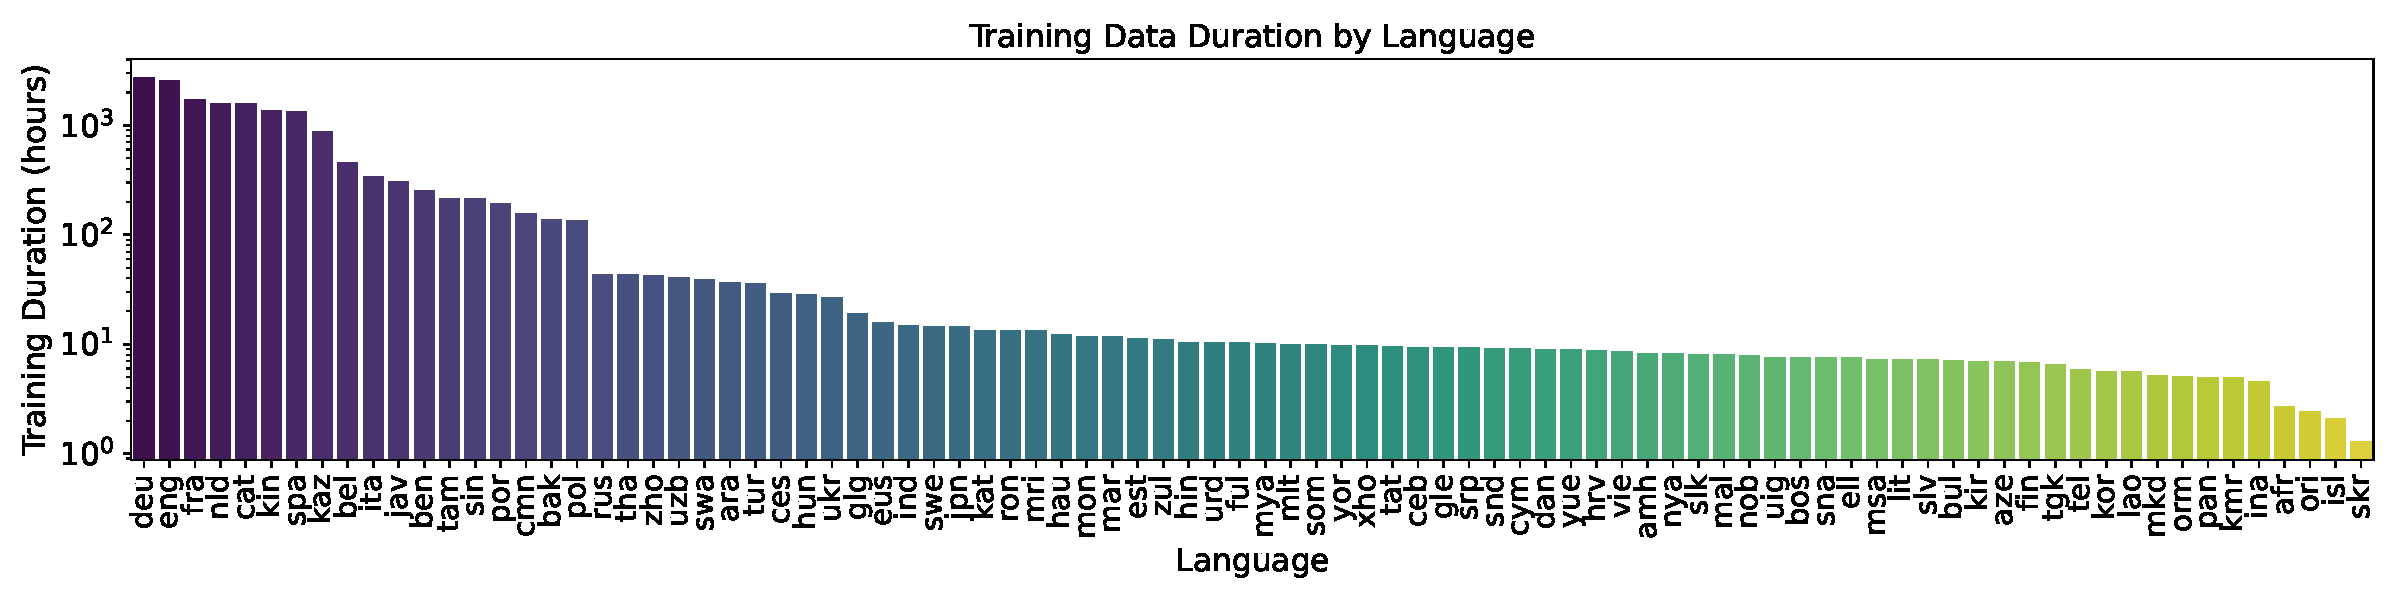
\includegraphics[width=\linewidth]{Figures/lang_distribution.pdf}
    \caption{The distribution of labeled training data duration by language, totaling 17,132 hours.}
    \label{fig:dist}
\end{figure*}






\section{Data} \label{sec:data}
First, we have created \textsc{IpaPack++}, one of the largest phone-based speech corpora in 88 languages, totaling 17,132 hours. %The sources include Common Voice 16.0 \cite{ardila-etal-2020-common} and the IPA PACK \cite{zhu-etal-2024-taste}. 
While the original \textsc{Ipa Pack} \cite{zhu-etal-2024-taste} provides 2000+ hours of speech in 100+ languages, upon careful inspection, we noticed several shortcomings. First, the IPA transcriptions were not normalized across the corpus, such that different Unicode encodings were present for the same phone. Some non-IPA Unicode symbols were also present due to artifacts in preprocessing. Second, the original dataset was more suitable for keyword spotting than ASR as half of the corpus was short clips of words taken from continuous recordings. 

\subsection{Data selection}
To address some of these limitations and expand our efforts, we have created a large-scale speech dataset for phone recognition. The datasets are recreated from \textsc{Ipa Pack} \cite{zhu-etal-2024-taste}, Common Voice 16.0 \cite{ardila-etal-2020-common}, LibriSpeech \cite{panayotov2015librispeech}, Multilingual LibriSpeech \cite{pratap20_interspeech}, Aishell-1 \cite{bu2017aishell}, crowd-sourced speech corpora for Javanese, Sinhala, and Bengali \cite{kjartansson-etal-sltu2018}, IISc-MILE Tamil ASR Corpus \cite{mile_1,mile_2}, Kazakh Speech Dataset \cite{mansurova-kadyrbek-2023-kazakh-speech-dataset} and Kazakh Speech Corpus \cite{khassanov-etal-2021-crowdsourced}. CharsiuG2P \cite{zhu22_interspeech} and Epitran \cite{mortensen-etal-2018-epitran} were used to automatically create phonemic transcriptions of available languages. 

After preprocessing, we ended up with around 17,135 hours of training data with G2P-generated transcriptions in 88 languages. The language distribution of the \textsc{IpaPack++} is shown at Figure~\ref{fig:dist}. A complete breakdown of individual languages can be found in Appendix~\ref{app:dataset}.


\begin{table*}[]
\small
\centering
\resizebox{\textwidth}{!}{%
\begin{tabular}{lrl}
\toprule
Dataset    & Dur. & Description \\\midrule
\texttt{Doreco}     & 19 hrs      & 45 languages collected and transcribed by field linguists.     \\
\texttt{VoxAngeles} & 1.5 hrs     & A set of individual word recordings from 95 languages.  \\\midrule
\texttt{Buckeye}    & 8 hrs & A collection of sociolinguistic recordings, carefully annotated by trained phoneticians. \\
\texttt{L2-Standard} & 4 hrs & L2-ARCTIC speech corpus with dictionary-based phonetic transcriptions. \\
\texttt{L2-Perceived} & 4 hrs & L2-ARCTIC speech corpus with human transcriptions of the actual pronunciation. \\\midrule
\texttt{Seen languages} & 65 hrs & Test sets from Aishell, LibriSpeech, and the Multilingual LibriSpeech (except for English). \\
\bottomrule
\end{tabular}%
}
\caption{A list of the evaluation datasets. These datasets cover a wide range of languages and sociophonetic conditions. }
\label{tab: eval_dataset}
\end{table*}


\subsection{Tokenization} 
The prior state-of-the-art universal phone recognizer \cite{xu22b_interspeech} adopted a data-driven approach to tokenization. However, this approach is not without problems. The phone tokenizer includes plain phones as well as phone combinations that are highly language-specific. For example, it uses a numerical representation of Mandarin tones rather than the standard IPA tone notations, also known as Chao tone letters. The numerical representation represents symbolic phonological contrasts of the tones, whereas the Chao tone letters reflect aspects of the phonetic realization like the f0 contour. Overall, though, using inconsistent symbols can limit knowledge sharing across languages \cite{zhu-etal-2024-taste}. 

We further made a systematic effort to normalize IPA encodings. In the first round of filtering, PHOIBLE \cite{moran2014phoible} was used as a reference to determine whether a phone was legitimate. Illegitimate phones were corrected: 1) phones with more than 3 diacritics can be overly complex to transcribe, so they are simplified to no more than one; 2) phones with inconsistent Unicode encodings, such as [g] (Unicode: U+0067) and [\textipa{g}] (Unicode: U+0261), are unified in one representation. Since we only focused on broad transcriptions, our final tokenizer only consists of all individual IPA symbols and the 15 most frequent diacritics from the IPA chart. Each diacritic is encoded as a separate token to reduce the vocabulary size. 



\subsection{Evaluation set}
\paragraph{Evaluating on seen languages}
We used the test set of several publicly available datasets to evaluate model performance. The G2P-generated phone transcriptions are quite noisy \citep{samir2024efficiently}, especially for low-resource languages. Therefore, we selected the test sets from Aishell-1 \cite{bu2017aishell}, Librispeech \cite{panayotov2015librispeech} and Multilingual LibriSpeech (MLS) \cite{pratap20_interspeech}, where the phone transcription quality was determined to be good upon our inspection. 

\paragraph{Evaluating on unseen languages}
In order to test how universal phone recognition models generalize across languages, we reserved the VoxAngeles \cite{chodroff-etal-2024-phonetic}, a clean version of the UCLA Phonetic Corpus \cite{li2021multilingual}, and DoReCo \cite{paschen2020building} for evaluation on unseen languages. Both datasets consist of speech recordings collected from fieldwork and transcribed phonetically by trained linguists. 

\paragraph{Evaluating on sociophonetic variation}
Most phone recognition models are trained and evaluated on dictionary pronunciations generated from pronunciation dictionaries and G2P models. These training and evaluation data might not reflect the actual pronunciation in spontaneous speech. We also measure how phone recognition models can predict actual phonetic variation. Such evaluation can serve to assess whether phone recognition models are suitable for tasks like pronunciation assessment and sociophonetic transcriptions. 

Here we utilize L2 ARCTIC \cite{zhao2018l2} and the Buckeye Corpus \cite{pitt2005buckeye}, both of which contain highly variable English speech carefully transcribed by professional linguists. For the Buckeye Corpus, we segmented all recording files into individual utterances between 20 to 50 phonemes, delimited by silent intervals ($\geq 200$ms) \cite{fuchs22_interspeech}. For L2 ARCTIC, we used the original segmentation but generated two versions of transcriptions, one for dictionary pronunciations of the prompts and one for the perceived pronunciations annotated by linguists. 


\section{Method}
Some prior studies in universal phone recognition  leverage knowledge of the language's phonemic inventory \cite{li2020universal,glocker23_interspeech}. However, the inventory is a static, abstract description of the phonological system of a language, only capturing a limited, idealized variation of speech. Many speech variations within a language can go beyond the inventory. In many applications of phone recognition such as pathological speech assessment, pronunciation assessment, and sociophonetics, transcribing speech into phones as it is actually articulated is important. Therefore, in our proposed models, we did not directly incorporate language-specific inventory knowledge, noting that such knowledge can also be incorporated in post-processing \cite{xu22b_interspeech}. 


\subsection{Zipformer}
Pretrained self-supervised models such as XLS-R \cite{babu22_interspeech} and Whisper \cite{radford2023robust} have been utilized as base models for fine-tuning in prior studies \cite{xu22b_interspeech,taguchi23_interspeech,glocker23_interspeech,samir2024efficiently}.
However, fine-tuning these transformer models on our large-scale dataset is prohibitively expensive with an academic computing budget. For example, Whisper pads every input utterance, regardless of their lengths, to chunks of 30 seconds,  allocating many computations to padding tokens that do not contribute to inference. Moreover, its autoregressive decoding is also highly inefficient.

Instead, we adopt Zipformer \citep{yao2023zipformer}, a transformer encoder model with U-Net style downsampling and upsampling layers \cite{ronneberger2015u} as the base architecture. Compared to the vanilla transformers (e.g., Wav2Vec2 and XLS-R), Conformer \cite{gulati20_interspeech}, Branchformer \cite{peng2022branchformer} and E-Branchformer \cite{kim2023branchformer}, Zipformer has demonstrated superior ASR performance with less compute \citep{yao2023zipformer}. Zipformer achieves such compute efficiency through reusing attention weights across layers, and progressively downsampling speech in the middle layers and upsampling to the output resolution in later layers. 

\subsection{CR-CTC}
%\subsection{Mixture of expert layers}
%We augmented Zipformers by replacing their feedforward layers with the MoE layers. MoE layers can effectively increase the model parameters without increasing the inference costs as much \cite{shazeer2016outrageously,riquelme2021scaling,gale2023megablocks}. 
We use the Connectionist Temporal Classification (CTC) loss \cite{graves2006connectionist} because it enables efficiently parallelized predictions and has maintained competitive results compared to an encoder-decoder architecture \cite{peng2024owsm}. Specifically, we adopted Consistency-Regularized CTC \cite{yao2025crctc} for our phone recognition model. 

Given a speech-transcription pair $(\mathbf{x},\mathbf{y})$, we fit an ASR model $f(\cdot)$. For the input speech spectrogram $\mathbf{x}$, $\mathbf{x}^{(a)}$ and $\mathbf{x}^{(b)}$ are two different augmented views generated through SpecAugment \cite{park19e_interspeech}. Two CTC output frame-wise distributions are generated through $\mathbf{z}^{(a)}=f(\mathbf{x}^{(a)})$ and $\mathbf{z}^{(b)}=f(\mathbf{x}^{(b)})$. 
Then the CR-CTC loss is formulated as:
\begin{align*}
\mathcal{L}_{CR-CTC} &= \frac{1}{2}\left( \mathcal{L}_{CTC}(\mathbf{z}^{(a)}, \mathbf{y}) + \mathcal{L}_{CTC}(\mathbf{z}^{(b)}, \mathbf{y}) \right) \\
            &\quad + \alpha \mathcal{L}_{CR}(\mathbf{z}^{(a)}, \mathbf{z}^{(b)})
\end{align*}
In addition to the regular CTC loss $\mathcal{L}_{CTC}$, $\mathcal{L}_{CR}$ is used to regularize the output distributions with Kullback-Leibler (KL) divergence between two frame-wise distributions at the same time step. The CR loss is defined as:
\begin{align*}
\mathcal{L}_{CR}(\mathbf{z}^{(a)}, \mathbf{z}^{(b)}) &= \frac{1}{2}\sum_{t=1}^{T}D_{KL}\left(sg(z_t^{(b)}),z_t^{(a)}\right) \\
            &\quad + D_{KL}\left(sg(z_t^{(a)}),z_t^{(b)}\right)
\end{align*}
where $sg(\cdot)$ is the stop-gradient operation and $D_{KL}$ is the KL divergence. $\mathcal{L}_{CR}$ performs self-distillation between outputs of two different augmented input views, mitigating overfitting. It has been shown to outperform regular CTC loss and RNN-T loss \cite{yao2025crctc}. 

We used the original CR-CTC implementation \cite{yao2025crctc} with minor modifications. The output temporal resolution is 25 Hz in the original Zipformer model. Yet this resolution is too short for phone sequences, which are significantly longer than text tokens. We upsampled the output resolution to 50 Hz to present numerical errors when computing the CTC loss. We also trained two variants of CR-CTC models: \textsc{Zipa-Cr-small} with 64M parameters and \textsc{Zipa-Cr-large} with 300M parameters. 




\subsection{Transducer}
We also trained Zipformer-based transducer models \citep{yao2023zipformer}. The original RNN-T loss for tranducers is computation- and memory-intensive, so we utilized the memory-efficient pruned RNN-T loss \cite{kuang22_interspeech}. In the transducer, we used Zipfomer as the encoder and the stateless decoder with 1D convolutional layers \cite{ghodsi2020rnn}. We trained two variants with non-causual attention: \textsc{Zipa-t-small} with 65M parameters and \textsc{Zipa-t-large} with 302M parameters. 

\subsection{Noisy student training}
Prior studies have shown that noisy student training \cite{park20d_interspeech}, or training on pseudo-labels can reliably improve multilingual ASR performance \cite{hwang2022large,hwang22c_interspeech,ramirez2024anatomy}. We generated phone pseudo-labels for two unannotated multilingual speech datasets, VoxLingua-107 and MMS ulab v2. VoxLingua-107 \cite{valk2021voxlingua107} consists of speech recordings without transcriptions from 107 languages, totaling 6,628 hours. MMS ulab v2 \cite{chen-etal-2024-towards-robust} is a 6,700-hour speech dataset in 4,023 languages, a reproduction of the original dataset for training Meta MMS \cite{pratap2024scaling}. As our labelled training data only included 88 unique languages, these two datasets can tremendously enrich the language diversity of our training data. 

We used all four Zipformer-based phone recognition models to generate the pseudo-labels for these two multilingual corpora, and computed the pairwise Phonetic Feature Error Rate (PFER) with PanPhon \cite{mortensen-etal-2016-panphon}. The consistencies of predictions between models were used as a heuristic to filter out bad predictions. Speech samples with an averaged pairwise PFER higher than the 80 percentile were ultimately excluded. We used pseudo-labels from \textsc{Zipa-Cr-large} as the final transcriptions for simplicity. Finally, we obtained pseudo-labels for 11,851 hours of multilingual speech in around 4,000 languages. We continued to train the CR-CTC models by mixing both the original dataset and pseudo-labelled dataset. The loss function was formulated as below.
$$
\mathcal{L}_{mixed} = \mathcal{L}_{CR-CTC} + \lambda\cdot\mathcal{L}_{CR-CTC}^{Pseudo}
$$
The hyperparameter $\lambda$ was set to 0.5 to downscale the weights of the noisy pseudo-labels. We adopted noisy student training to train \textsc{Zipa-Cr-Ns-small} and \textsc{Zipa-Cr-Ns-large}, both of which were initialized from pretrained checkpoints of \textsc{Zipa-Cr-small} and \textsc{Zipa-Cr-large} respectively. 

\paragraph{No-Diacritic Models} Our error analysis suggested that many recognition errors were associated with diacritics. During noisy student training, we also trained two variants of  \textsc{Zipa-Cr-small} and \textsc{Zipa-Cr-large} without diacritics. We maintained the exact same training settings, but removed all diacritics from all training data. For consistency, these models were also evaluated with the same evaluation data but without diacritics.  

\begin{table*}[]
\centering
\small
\resizebox{\textwidth}{!}{%
\begin{tabular}{rrcrrrrrrrrrr}
\toprule
Model & Param. & Iters & \texttt{eng-c} & \texttt{eng-o} & \texttt{ger} & \texttt{por} & \texttt{fre} & \texttt{spa} & \texttt{dut} & \texttt{ita} & \texttt{cmn} & \texttt{Avg.}\\\midrule
\texttt{Allosaurus}      &     11M       &      -     &    4.18       &  6.21   &  30.26  &  33.09 &  32.77    &  28.02  & 33.29 & 26.57 & 6.64  & 22.33 \\
\texttt{W2V2P-lv-60-ft} & 300M & - & 4.09 & 4.26 & 18.11 & 23.47 &  28.63   &  7.97 & 27.27  & 8.63 &  6.82 & 14.36\\
\texttt{W2V2P-xlsr-53-ft}       &     300M       &    -       &    5.45       &     5.35   &   11.61  &  18.80   &  26.59   &  5.14 & 20.91 & 6.93 & 6.20 & 11.88  \\
\texttt{MultIPA}$^*$      &   300M         &    -       &   11.26        &  10.86   &  27.02   &  25.05   &   31.31  &  12.02   & 32.15 & 11.22 & 8.35 & 18.80 \\
\texttt{WhisperPPT} & 244M & - & 6.36 & 7.39 & 20.40 & 18.29 & 26.85 & 6.89 & 13.29 &  5.52 & 2.03 & 11.89 \\\midrule
\textsc{Zipa-T-small}     &    65M        &    300k               & 1.17    &  2.14   &  4.66   &  18.20   &  16.68  &  2.34 & 6.84 & 5.05 & 0.72 & 6.42  \\
\textsc{Zipa-T-large}     &     302M       &   300k        &     0.70     &  1.35   &  3.76   &  6.52   &  5.32   &   1.85  &  5.33 & 8.91 & 0.52 & 3.80 \\
\textsc{Zipa-T-small}     &    65M        &    500k       &      0.95     &  1.67   & 3.51    &   17.01  &  7.49   & 2.08 &  5.49   & 2.66 & 0.78  & 4.62  \\
\textsc{Zipa-T-large}     &     302M       &    500k       &       \textbf{0.61}   &  \textbf{1.19}   &   3.38  &   \underline{5.96}  &  \textbf{4.52}   &  \textbf{1.69}   & \textbf{4.62}  & \textbf{1.91} & \underline{0.44} & \textbf{2.70}  \\\midrule
\textsc{Zipa-Cr-small}     &     64M       &    300k      & 2.36    &  3.29   &  14.11   &  20.19   &  18.19   &  4.07 & 9.69 & 8.27 & 1.59  & 9.08  \\
\textsc{Zipa-Cr-large}     &     300M       &    300k       &     1.07      &   1.92  &   3.70  &  21.15   &  5.47   & 2.37    &   5.25 &  2.28 & 0.55 & 4.86 \\
\textsc{Zipa-Cr-small}     &     64M       &     500k      &      1.15     &  2.23   &  3.56   &  18.19   & 6.13    &  2.74   &  7.27 & 8.47& 0.84 & 5.62  \\
\textsc{Zipa-Cr-large}     &     300M       &    500k       &      0.77     &  1.49   & \underline{3.34}    &  7.10   &  4.99   &  2.58   & 5.23  & 2.23& 0.54 & 3.14 \\\midrule
%\textsc{Zipa-Cr-l}     &     300M       &    800k       &      0.69     &  1.33   & 2.86    &  8.33   &  5.24   &  1.76   & 5.31  & 2.74 & 0.40  \\\midrule
\textsc{Zipa-Cr-Ns-small}     &     64M       &     700k      &  0.75 &  1.51 &  3.41 & 8.56 & 4.87 & 2.36 &  4.9 & \underline{2.19} & 0.50 & 3.22 \\
\textsc{Zipa-Cr-Ns-large}     &     300M       &    800k       &  \underline{0.66} & \underline{1.29} & \textbf{3.07} & \textbf{5.47} &  \underline{4.53} & \underline{1.98} & \underline{4.86} & 2.23 & \textbf{0.38}  & \underline{2.71}   \\\midrule
\textit{No diacritics$^{**}$} \\\midrule
\textsc{Zipa-Cr-Ns-small}     &     64M       &     700k      &  0.78 &  1.51 &  3.25 & 8.70 & 4.83 & 2.31 &  4.73 & 2.10 & 0.50 & 3.02 \\
\textsc{Zipa-Cr-Ns-large}     &     300M       &    780k       &  0.65 & 1.28 & 2.95 & 4.92 &  4.55 & 2.24 & 4.68 & 2.20 & 0.41  & 2.65   \\
\bottomrule
\end{tabular}
}
\caption{Main PFER results on seen languages. $^*$Some languages were not seen by \texttt{MultiIPA}. $^{**}$Diacritics were removed for both training and evaluation sets, so results are not directly comparable with other models. \textbf{Notations:} \textsc{T} - Transducer; \textsc{Cr} - Consistency-regularized CTC; \textsc{Ns} - Noisy student training. }
\label{tab:seen}
\end{table*}

\section{Experiments}

\subsection{Implementation} Our experiments were structured within the Next-gen Kaldi framework. We used \texttt{lhotse}\footnote{\url{https://github.com/lhotse-speech/lhotse}} to manage data loading and augmentation, \texttt{icefall}\footnote{\url{https://github.com/k2-fsa/icefall}} for training and evaluation, and \texttt{k2}\footnote{\url{https://github.com/k2-fsa/k2}} for the pruned transducer loss. The inputs to all models are the 80-dimensional Mel Frequency Cepstral Coefficients (MFCCs).
We used the Scaled Adam optimizer, which was shown to work better with Zipformer than Adam \citep{yao2023zipformer}. All models were trained from scratch with randomly initialized weights. During evaluation, the final model for each variant was the averaged model from the last 10 checkpoints. Simple greedy decoding was used to generate predictions in all conditions. We trained all small models with an A40 40G GPU and all large models with 2 A100 40G GPUs. 
Detailed hyperparamters are described in Appendix~\ref{app:training}.


\begin{table*}[]
\small
\centering
\resizebox{\textwidth}{!}{%
\begin{tabular}{@{\extracolsep{4pt}}rcrrrrrrr}
\toprule
\multirow{2}{*}{Model} & \multirow{2}{*}{Param.} & \multirow{2}{*}{Iters}  & \multicolumn{2}{c}{\bf Unseen} & \multicolumn{3}{c}{\bf Sociophonetic} & \multirow{2}{*}{Avg.} \\\cline{4-5}\cline{6-8}
                       &                             &                        & \texttt{Doreco}     & \texttt{VoxAngeles}    & \texttt{L2-Standard}  & \texttt{L2-Perceived}      & \texttt{Buckeye}       \\\midrule
\texttt{Allosaurus}      &     11M       &    -       &  8.89         &   1.35 &  5.21 & 5.72 & 5.04 & 5.24 \\
\texttt{W2V2P-lv-60-ft} & 300M & - & 6.13 & 0.66 & 2.89 & 3.95 & \textbf{3.85} & 3.49 \\
\texttt{W2V2P-xlsr-53-ft}      &     300M       &    -       &  \underline{5.94}    &  \textbf{0.58}    &  3.69 & 4.09   &      3.97 & 3.65 \\
\texttt{MultIPA}      &   300M         &     -      &    6.55       &  \underline{0.62}    & 5.86 & 5.88 & 5.94 & 4.97   \\
\texttt{WhisperPPT} & 244M & - & 9.31 & 0.91 & 6.44 & 6.65 & 6.80 & 6.02 \\\midrule
\textsc{Zipa-T-small}     &    65M        &   300k               &  7.20 & 0.71 & 2.26 & 3.85 & 4.00 & 3.60     \\
\textsc{Zipa-T-large}     &     302M       &     300k      &       7.27     &   0.88   & 1.79 & 3.67 & 3.95 & 3.51\\
\textsc{Zipa-T-small}     &    65M        &     500k      &       8.72    &    0.78  &  1.99 & 3.80 & 3.97 & 3.85  \\
\textsc{Zipa-T-large}     &     302M       &    500k       &        8.05    &  0.88   &  \textbf{1.68} & \textbf{3.63} & 3.94 & 3.63 \\\midrule
\textsc{Zipa-Cr-small}     &     64M       &    300k        &  5.97 & 0.78 & 3.42 & 5.13 & 4.58  & 3.97    \\
\textsc{Zipa-Cr-large}     &     300M       &   300k        &     6.90      &    0.83  & 2.15 & 3.71 & 3.91 & 3.50 \\
\textsc{Zipa-Cr-small}     &     64M       &    500k       &    6.02       &   0.65  &   2.54 & 4.60 & 4.71 & 3.70    \\
\textsc{Zipa-Cr-large}     &     300M       &   500k        &      6.37     &   0.77  & 1.87 &  3.69  & 3.93 & 3.32 \\\midrule 
%\textsc{Zipa-Cr-l}     &     300M       &   800k        &      6.10     &   0.78  & 1.81 &  3.74  & 3.97  \\ \midrule
\textsc{Zipa-Cr-Ns-small}     &     64M       &    700k       &    \underline{5.94}       &   0.69  &   1.94 & 3.79 & \underline{3.87}  & \underline{3.24}   \\
\textsc{Zipa-Cr-Ns-large}     &     300M       &   800k        &  \textbf{5.93} & 0.75 &  \underline{1.75} & \underline{3.67} & 3.92  & \textbf{3.20} \\ \midrule
\textit{No diacritics$^{**}$} \\\midrule
\textsc{Zipa-Cr-Ns-small}     &     64M       &    700k       &   5.80       &   0.68  &   1.92 & 3.76 & 3.86  & 3.21   \\
\textsc{Zipa-Cr-Ns-large}     &     300M       &   780k        &  5.81 & 0.71 &  1.78 & 3.66 & 3.86  & 3.17 \\ 
\bottomrule       
\end{tabular}
}
\caption{Main PFER results on unseen languages and domains. $^{**}$Diacritics were removed for both training and evaluation sets, so results are not directly comparable with other models. \textbf{Notations:} \textsc{T} - Transducer; \textsc{Cr} - Consistency-regularized CTC; \textsc{Ns} - Noisy student training.}
\label{tab:unseen}
\end{table*}


\subsection{Baselines}
To contextualize the performance of the proposed model, we compared our models with several universal phone recognition models with publicly available weights. 
\begin{itemize}
    %\setlength{\itemsep}{0pt}  % Reduce space between items
    \setlength{\parskip}{1pt}  % Remove extra space between 
    \item \textbf{Allosaurus}. Allosaurus \cite{li2020universal} is one of the earliest universal phone recognizers. The network backbone consists of bi-directional LSTM networks, and it has a shared phone output layers and language-specific allophone layers. 
    \item \textbf{Wav2Vec2Phoneme}. Wav2Vec2Phoneme \cite{xu22b_interspeech} is a state-of-the-art phone recognizer based on the pretrained Wav2Vec2 and XLSR-53 model \cite{baevski2020wav2vec,conneau2020unsupervised}. It was fine-tuned on 57k hours of speech data with phone transcriptions. We examined two checkpoints: \texttt{W2V2P-lv-60-ft}\footnote{\url{https://huggingface.co/facebook/wav2vec2-lv-60-espeak-cv-ft}}, which was fine-tuned from Wav2Vec2, and \texttt{W2V2P-xlsr-53-ft}\footnote{\url{https://huggingface.co/facebook/wav2vec2-xlsr-53-espeak-cv-ft}}, which was initialized with XLSR-53. 
    \item \textbf{MultIPA}. MultIPA\footnote{\url{https://huggingface.co/ctaguchi/wav2vec2-large-xlsr-japlmthufielta-ipa1000-ns}} \cite{taguchi23_interspeech} is another model based on the XLSR-53 \cite{conneau2020unsupervised}. The model was fine-tuned on relatively small but high-quality data with phone transcriptions, achieving competitive performance in phone recognition. 
    \item \textbf{Whisper-PPT}. Whisper-PPT \cite{samir2024efficiently} is an autoregressive universal phone recognition model based on the pretrained \texttt{Whisper-small} \cite{radford2023robust}. It was fine-tuned on a selected high-quality subset of IPAPack \cite{zhu-etal-2024-taste}. Unlike other models, the autoregressive nature of Whisper makes it uniquely prone to repeatedly generating hallucinated substrings on occasion.  
\end{itemize}
Allophant \cite{glocker23_interspeech} is another state-of-the-art phone recognizer based on XLS-R \cite{babu22_interspeech}. However, Allophant relies on an existing phoneset to make predictions. Some of our evaluation datasets, such as unseen languages and L2 speech, do not have an existing phoneset in PHOIBLE, so we did not compare with Allophant. 



\section{Results}
We evaluated model performance with the PFER, which measures the alignment of binary articulatory features. The metric was computed with PanPhon \cite{mortensen-etal-2016-panphon}. The main results are presented in Table~\ref{tab:seen} and Table~\ref{tab:unseen}. Below we summarize our main findings. 

\paragraph{ZIPA models reach state-of-the-art performance on multilingual phone recognition.} We trained \textsc{Zipa} variants on 17k hours of multilingual data from scratch. Even the small \textsc{Zipa} models with only 64M parameters can outperform the 300M transformer baselines that have been pretrained and/or fine-tuned on much more data. For example, both \texttt{FAIR-lv-60-ft} and \texttt{FAIR-xlsr-60-ft} \cite{xu22b_interspeech} were initialized from pretrained weights and fine-tuned on 57k labeled data. Meanwhile, the Zipformer backbone is also much more memory efficient and less computationally intensive than the vanilla transformer in XLSR series of models and Whisper \cite{yao2023zipformer}. Our study shows that careful curation of data, including increasing data quantity and carefully normalizing the IPA labels, as well as a good choice of backbone model can yield effective improvement.  

\paragraph{Smaller models and non-autoregressive models generalize better to unseen languages but perform worse on seen languages.} 

Our results show that transducer models tend to outperform CTC based models on seen languages (see Table~\ref{tab:seen}). Autoregressive transducers model the dependencies better than CTC models, where conditional independence between labels is learned. However, learning the causal dependencies between phones can also hurt the multilingual generalizability, as unseen languages might have a different phonological structure. 
Larger models also tend to overfit the training data, weakening their abilities to predict unseen languages. This is particularly evident on both \texttt{Doreco} and the \texttt{VoxAngeles} test sets.  

Yet CTC models are still valuable as they are more efficient than autoregressive models and can be combined with an external alignment algorithm to generate approximate time stamps for multilingual data \cite{kurzinger2020ctc, pratap2024scaling}.

It is important to note that the evaluation metric PFER is a distance function rather than a ratio, so its magnitude tends to correlate with length. While it appears that the PFER for seen languages (Table~\ref{tab:seen}) is higher than the PFER for unseen languages (Table~\ref{tab:unseen}), it is because the speech samples from seen languages are longer than those from unseen languages. In Table~\ref{tab:seen}, some languages, especially \texttt{por} and \texttt{fre}, have consistently lower scores than other languages. This is caused by both the length of the evaluation samples and the phone set mismatch in these languages. For example, Portuguese uses [\textipa{5}] frequently but it is often transcribed as the more crosslinguistically frequent [a]. French marks nasality with a diacritic [\textasciitilde], but other languages tend to use the nasal consonants. Such mismatches in the phone set pose challenges to the phone recognition system, especially for small models. Yet longer training time and more model parameters enable models to memorize these language-specific conventions better. At least for high-resource languages, ZIPA models can implicitly distinguish the language and transcribe phones accordingly. 


\begin{table}[]
\centering
\small
\begin{tabular}{lrr}
\toprule
Model & Seen Avg. & Unseen Avg. \\\midrule
\textsc{Zipa-Cr-l} \\
\hspace{0.2in} - 800k &   3.18        &    3.28         \\
\textsc{Zipa-Cr-Ns-l}     &           &    \\
\hspace{0.2in} - $\lambda$=0.5 & \textbf{2.71} & 3.20 \\
\hspace{0.2in} - $\lambda$=1.0 & 2.77 & \textbf{3.19} \\\midrule
\textsc{Zipa-Cr-Ns-s}     &           &            \\
\hspace{0.2in} - $\lambda$=0.2 &  3.36 & 3.35\\
\hspace{0.2in} - $\lambda$=0.5 & \textbf{3.22} & 3.24\\
\hspace{0.2in} - $\lambda$=1.0 & 3.41 & \textbf{3.23} \\\bottomrule
\end{tabular}
\caption{Ablation analysis of noisy student training.}
\label{tab: abation}
\end{table}




\paragraph{Noisy student training brings minor but consistent improvement.} \textsc{Zipa-Cr-Ns} models can consistently improve model performance, though the improvement is minor. This is likely because the pseudo-labels on unseen languages are extremely noisy, diminishing the benefits of additional data. Our ablation analysis in Table~\ref{tab: abation} indicates that continuing to train together with pseudo-labelled data is more beneficial than continuing to train on the existing labeled data beyond 500k steps. The value of $\lambda$ seems to control the trade-off between in-domain and out-of-domain performance, but the overall impact of $\lambda$ is not large. Note that we only adopted a simple approach to do noisy student training, so there is still room for improvement. Further research is needed to investigate how to better exploit the massive amount of unlabelled data. 


\begin{figure*}
    \centering
    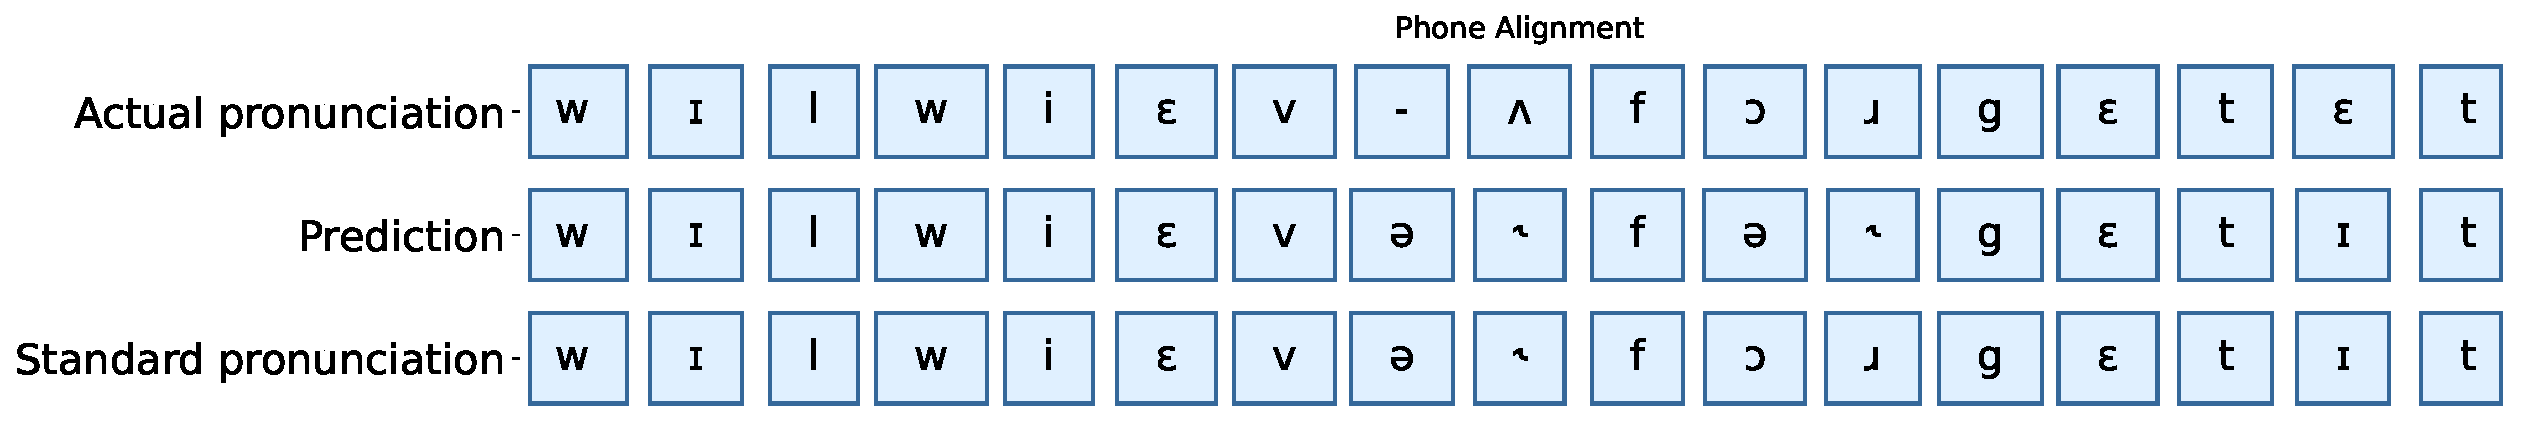
\includegraphics[width=\linewidth]{Figures/triple_alignment.pdf}
    \caption{A sample transcription of the prompt ``\textit{Will we ever forget it}" in L2 speech by \textsc{Zipa-Cr-Ns-l}. The predicted transcription aligns more with the standard pronunciation, suggesting that the model failed to capture the actual sociophonetic variation. }
    \label{fig:alignment}
\end{figure*}

\begin{figure}
    \centering
    
\includegraphics[width=\linewidth]{Figures/error.pdf}
    \caption{Distributions of transcription error types. Substitution errors are most common across models. Transducers exhibit a relatively high rate of deletion errors.}
    \label{fig:error_type}
\end{figure}


\begin{table}
\small
\centering
\begin{minipage}{0.3\linewidth}
    \begin{tabular}{cc}
    \toprule
    \textbf{IPA} & \textbf{Del} \\
    \midrule
    \textipa{:} & 17225 \\
    \textipa{P} & 11105 \\
    \textipa{i} & 7172 \\
    \textipa{a} & 5631 \\
    \textipa{n} & 4714 \\
    \textipa{h} & 4204 \\
    \textipa{e} & 3727 \\
    \textipa{E} & 3646 \\
    \textipa{u} & 3399 \\
     \textasciitilde & 3249 \\
    \textipa{o} & 3232 \\
    \textipa{t} & 2492 \\
    \textipa{@} & 2291 \\
    \textipa{I} & 2041 \\
    \textipa{w} & 1965 \\
    \textipa{j} & 1938 \\
    \textipa{d} & 1811 \\
    \textipa{k} & 1647 \\
    \textipa{O} & 1612 \\
    \textipa{\super h} & 1505 \\
    \bottomrule
    \end{tabular}
\end{minipage}%
\hspace{0.3cm} 
\begin{minipage}{0.3\linewidth}
    \begin{tabular}{cc}
    \toprule
    \textbf{IPA} & \textbf{Ins} \\
    \midrule
    \textipa{:} & 9777 \\
    \textipa{\|[c}$^*$ & 3924 \\
    \textipa{a} & 3401 \\
    \textipa{j} & 2793 \\
    \textipa{i} & 2491 \\
    \textipa{u} & 2123 \\
    \textipa{e} & 1943 \\
    \textipa{t} & 1487 \\
    \textipa{k} & 1487 \\
    \textipa{S} & 1414 \\
    \textipa{Z} & 1289 \\
    \textipa{n} & 1265 \\
    \textipa{U} & 894 \\
    \textipa{o} & 814 \\
    \textipa{p} & 781 \\
    \textipa{w} & 759 \\
    \textipa{@} & 696 \\
    \textipa{r} & 667 \\
    \textipa{d} & 653 \\
    \textipa{R} & 648 \\
    \bottomrule
    \end{tabular}
\end{minipage}%
\hspace{0.3cm} 
\begin{minipage}{0.3\linewidth}
    \begin{tabular}{cc}
    \toprule
    \textbf{IPA} & \textbf{Sub} \\
    \midrule
    \textipa{a} $\to$ \textipa{A} & 5669 \\
    \textipa{i} $\to$ \textipa{e} & 5592 \\
    \textipa{E} $\to$ \textipa{e} & 4454 \\
    \textipa{o} $\to$ \textipa{u} & 3478 \\
    \textipa{e} $\to$ \textipa{i} & 3089 \\
    \textipa{u} $\to$ \textipa{o} & 2889 \\
    \textipa{O} $\to$ \textipa{o} & 2678 \\
    \textipa{E} $\to$ \textipa{a} & 2480 \\
    \textipa{@} $\to$ \textipa{a} & 2226 \\
    \textipa{e} $\to$ \textipa{a} & 1932 \\
    \textipa{b} $\to$ \textipa{p} & 1859 \\
    \textipa{d} $\to$ \textipa{t} & 1717 \\
    \textipa{o} $\to$ \textipa{O} & 1716 \\
    \textipa{i} $\to$ \textipa{j} & 1619 \\
    \textipa{g} $\to$ \textipa{k} & 1609 \\
    \textipa{o} $\to$ \textipa{a} & 1526 \\
    \textipa{i} $\to$ \textipa{I} & 1444 \\
    \textipa{E} $\to$ \textipa{e} & 1436 \\
    \textipa{r} $\to$ \textipa{R} & 1429 \\
    \textipa{e} $\to$ \textipa{E} & 1425 \\
    \bottomrule
    \end{tabular}
\end{minipage}
\caption{Summary of \textbf{Del}etions, \textbf{Ins}ertions, and \textbf{Sub}stitution errors by \textsc{Zipa-Cr-Ns-L}. Other \textsc{Zipa} models also exhibit a similar pattern. $^*$c denotes any consonant. }
\label{tab:errors}
\end{table}



\paragraph{Removing diacritics can improve the match between model predictions and ground truth, especially on unseen languages, but the impact is slight.} Both Table~\ref{tab:seen} and~\ref{tab:unseen} suggest that the no-diacritic condition yields inconsistent and slight improvement, as the number of total symbols is reduced. Our further inspection indicates that ZIPA models tend to handle diacritics pretty well for seen languages, as the patterns in these languages are probably well memorized during training. Yet, generalizing diacritics across languages poses a much larger challenge. The largest change in score is the \texttt{Doreco} evaluation set, as it contains more diacritics than other datasets \citep{paschen2020building}.


\section{Analysis} \label{sec:analysis}
We also conducted an error analysis to understand model behaviors and present findings below.
\paragraph{Phone recognition models tend to smooth out the phonetic variation during inference.}  In Table~\ref{tab:unseen}, there is a systematic gap between the performance of \texttt{L2-Standard} and the \texttt{L2-Perceived} test sets. In Figure~\ref{fig:alignment}, given the exact same L2 speech,  \textsc{Zipa} predictions tend to better match the standard dictionary pronunciation than the actual pronunciation. This is likely an artifact of data curation, as all of the training data were generated from pronunciation dictionaries and G2P models. Yet this finding also implies that the phone recognition models are still matching the frequent phone patterns in the dataset, rather than transcribing phones as they are actually produced. % Discuss more about. Tying results to specific experiments. Refer to specific columns and saying explicitly the difference between two architectures. 

\paragraph{Vowels are more difficult to predict crosslingusitically.} Prior research has revealed that certain sounds are recognized better across languages \cite{zelasko2022discovering}. We conducted an error analysis of the model predictions on \texttt{Doreco}. As shown in Figure~\ref{fig:error_type}, substitution errors are far more common than addition and deletion errors. Transducer models show much higher deletion errors than CTC models. Our close inspection also suggests that transducers generate quite a few empty transcriptions for unseen languages.  
% search phonetic literature

Table~\ref{tab:errors} provides further details on the top errors made by \textsc{Zipa-Cr-Ns}. The top deletion and insertion errors are diacritics. The length symbol \textipa{:} is consistently the most frequently added or deleted symbol, as vowel length is relative across languages. The glottal stop \textipa{P} is often not contrastive and not explicitly marked in IPA transcriptions, resulting in high deletions in model predictions. For substitution, the top errors are the substitution of vowels that are close in the vowel space. Compared to consonants, vowel realizations tend to be more gradient in their acoustics, resulting in higher acoustic overlap between otherwise contrastive vowel categories and therefore more ambiguous. Such misidentification patterns also mirror the patterns of human speech perception crosslinguistically \cite{sebastian2005cross}. 

%CTC-based models are more robust than transducers in unseen languages. Transducer models tend to predict all blanks for certain utterances in unseen languages. 
% Overrepresentation of English and German data might account for some of the errors. 
% Length is phonological rather than phonetic. Substitution errors are expected. b-d, g-k are inconsistent. All substituted sounds are on a continuum. Vowel space or VOT varies on a continuum. Model behaves reasonably. 

% Iterative refinement of the transcriptions. Use an external language model to rescore the output. This would be more helpful for linguists. 


%\section{LLM-assisted transcription}
%We conducted a case study to investigate how \textsc{Zipa} can be combined with an LLM to automate the phonetic transcription with phonetic knowledge. We collected 4022 recordings of 3616 unique Azerbaijani (\texttt{aze}) words from Lingua Libre\footnote{\url{https://lingualibre.org/wiki/LinguaLibre:Main_Page}}, a crowd-sourced website for word pronunciations. The IPA transcriptions were obtained from the pronunciation dictionaries from Epitran \cite{mortensen2018epitran}.

\section{Conclusions}
In conclusion, we present a large-scale multilingual phone recognition dataset \textsc{Ipa Pack++} and a series of Zipformer-based \textsc{Zipa} models, which exhibit state-of-the-art performance on phone recognition. We hope that our research can provide foundations to support more downstream multilingual speech processing tasks that benefit from phonetic transcriptions. Yet simply scaling up the G2P for transcribed speech data alone might not be able to solve phone recognition, as models can simply memorize the standard pronunciation. We will also actively explore how to incorporate more linguistic knowledge to further improve performance. 



\section*{Ethics statement}
We adhere to ethical practices in our research. We only selected publicly available datasets with permissive licenses that allow us to redistribute the processed data and the models. We believe that open-sourcing our research can help facilitate future research towards multilingual speech technologies for both the speech processing communities and the linguistics communities.

It is our firm belief that this research can contribute to the promotion of more inclusive speech technologies for more languages, especially for under-represented languages. While our model is primarily developed to support language documentation and other downstream applications, we are also aware that multilingual speech recognition can exhibit biases towards non-mainstream accents and potentially be used for malicious purposes such as surveillance. We urge that caution be exercised when deploying such models in downstream tasks. 

\section*{Limitations}
Our study is still limited in several ways. First, the number of languages studied in our paper is still limited. The distribution of languages is highly skewed in our dataset, which still biases our models towards high-resource languages. 

Secondly, our current approach trains models on synthetic labels from G2P. However, the data quality is limited as dictionary pronunciations might not reflect the actual pronunciation in spontaneous speech. This also results in the \textsc{Zipa} models to smooth out variation in some L2 speech. More research is needed to investigate how to curate higher quality data for phone recognition that can reflect the actual pronunciation. 

The limitation of computational resources also limits our abilities to perform extensive hyperparameter tuning and conduct extensive experiments to explore different architectures and pseudo-labeling strategies. In the future, we will continue to explore better strategies to continue to improve the performance of multilingual speech processing systems. 

\section*{Acknowledgments}
This research was enabled in part through the computational resources provided by Advanced Research Computing at the University of British Columbia and the Digital Research Alliance of Canada. FS is supported by an NSERC PGS-D Scholarship. The research activities were also supported by the NSERC Discovery Grant and the CFI JELF Grant awarded to JZ and by SNF Grant  PR00P1\_208460 to EC.

% Bibliography entries for the entire Anthology, followed by custom entries
%\bibliography{anthology,custom}
% Custom bibliography entries only
\bibliography{custom,anthology}

\appendix
\newpage
\onecolumn
\section{Dataset details}
\label{app:dataset}
\subsection{Dataset Overview}

{\centering{\small \begin{longtable}{cccc}
\toprule
Language & Split & Dataset & Total Duration \\ 
\midrule
swa & train & Common Voice & 28:48:36 \\ 
 & & Fleurs & 10:06:09 \\ \midrule
spa & train & Common Voice & 404:00:29 \\ 
 & & Fleurs & 06:43:33 \\ 
 & & Multilingual Librispeech & 917:41:03 \\ \midrule
bel & train & Common Voice & 452:08:22 \\ 
 & & Fleurs & 07:18:15 \\ \midrule
tam & train & Common Voice & 76:47:49 \\ 
 & & Fleurs & 06:20:35 \\ 
 & & IISc-MILE Tamil ASR Corpus & 133:17:27 \\ \midrule
kin & train & Common Voice & 1376:18:20 \\ \midrule
eng & train & Common Voice & 1584:30:15 \\ 
 & & Librispeech & 961:03:15 \\ 
 & & Fleurs & 05:38:28 \\ \midrule
ron & train & Common Voice & 05:44:05 \\ 
 & & Fleurs & 07:38:47 \\  \midrule
ell & train & Fleurs & 07:30:24 \\  \midrule
jpn & train & Fleurs & 05:03:22 \\ 
 & & Common Voice & 09:22:26 \\  \midrule
tur & train & Fleurs & 06:25:40 \\ 
 & & Common Voice & 29:30:44 \\ \midrule
hun & train & Common Voice & 21:15:06 \\ 
 & & Fleurs & 07:00:41 \\ \midrule
mon & train & Fleurs & 08:37:49 \\ 
 & & Common Voice & 03:13:37 \\ \midrule
ind & train & Common Voice & 07:46:52 \\ 
 & & Fleurs & 06:56:13 \\ \midrule
uig & train & Common Voice & 07:36:34 \\  \midrule
ita & train & Common Voice & 83:14:54 \\ 
 & & Fleurs & 06:51:31 \\ 
 & & Multilingual Librispeech & 247:22:40 \\  \midrule
mkd & train & Fleurs & 05:08:08 \\  \midrule
urd & train & Common Voice & 04:58:30 \\ 
 & & Fleurs & 05:20:32 \\ \midrule
vie & train & Fleurs & 06:42:36 \\ 
 & & Common Voice & 01:51:31 \\ \midrule
cat & train & Common Voice & 1591:25:03 \\ 
 & & Fleurs & 05:46:13 \\  \midrule
fra & train & Common Voice & 661:14:43 \\ 
 & & Multilingual Librispeech & 1076:34:49 \\ \midrule
mya & train & Fleurs & 10:04:25 \\  \midrule
kaz & train & Kazakh Speech Dataset  & 554:47:31 \\ 
 & & Kazakh Speech Corpus & 318:25:26 \\ 
 & & Fleurs & 08:54:35 \\  \midrule
deu & train & Common Voice & 778:17:18 \\ 
 & & Multilingual Librispeech & 1966:30:30 \\ 
 & & Fleurs & 06:52:51 \\  \midrule
kir & train & Fleurs & 06:59:30 \\ \midrule
mlt & train & Fleurs & 07:29:59 \\ 
 & & Common Voice & 02:24:53 \\  \midrule
bos & train & Fleurs & 07:34:14 \\  \midrule
srp & train & Common Voice & 01:08:08 \\ 
 & & Fleurs & 08:08:18 \\  \midrule
isl & train & Fleurs & 02:06:30 \\  \midrule
ori & train & Fleurs & 02:25:20 \\ \midrule
pol & train & Fleurs & 07:13:49 \\ 
 & & Multilingual Librispeech & 103:38:57 \\ 
 & & Common Voice & 24:47:44 \\ \midrule
nld & train & Common Voice & 38:07:31 \\ 
 & & Fleurs & 05:48:46 \\ 
 & & Multilingual Librispeech & 1554:14:38 \\ \midrule
slv & train & Fleurs & 05:46:47 \\ 
 & & Common Voice & 01:24:43 \\ \midrule
tel & train & Fleurs & 05:52:07 \\ \midrule
hin & train & Common Voice & 05:17:16 \\ 
 & & Fleurs & 05:08:23 \\  \midrule
ukr & train & Fleurs & 06:41:46 \\ 
 & & Common Voice & 19:56:08 \\  \midrule 
yor & train & Common Voice & 01:20:01 \\ 
 & & Fleurs & 08:27:42 \\ \midrule
aze & train & Fleurs & 06:53:37 \\  \midrule
zho & train & Common Voice & 42:04:06 \\ \midrule
mri & train & Fleurs & 13:20:08 \\ \midrule
rus & train & Fleurs & 06:16:41 \\ 
 & & Common Voice & 37:26:56 \\ \midrule
swe & train & Common Voice & 08:10:51 \\ 
 & & Fleurs & 06:20:35 \\ \midrule
pan & train & Fleurs & 04:57:37 \\  \midrule
mar & train & Common Voice & 02:13:16 \\ 
 & & Fleurs & 09:28:59 \\ \midrule
dan & train & Fleurs & 05:45:06 \\ 
 & & Common Voice & 03:16:57 \\ \midrule
zul & train & Fleurs & 11:03:07 \\  \midrule
nob & train & Fleurs & 07:57:37 \\  \midrule
por & train & Common Voice & 22:38:41 \\ 
 & & Multilingual Librispeech & 160:57:47 \\ 
 & & Fleurs & 07:45:54 \\ \midrule
ben & train & Crowd-sourced speech for Bengali & 215:24:21 \\ 
 & & Common Voice & 31:49:44 \\ 
 & & Fleurs & 08:10:49 \\ \midrule 
bak & train & Common Voice & 139:12:22 \\  \midrule
amh & train & Fleurs & 08:15:36 \\ \midrule
est & train & Fleurs & 05:22:55 \\ 
 & & Common Voice & 05:49:26 \\ \midrule
cmn & train & Aishell-1 & 150:50:14 \\ 
 & & Fleurs & 06:02:12 \\ \midrule
ces & train & Fleurs & 06:22:34 \\ 
 & & Common Voice & 22:25:29 \\  \midrule
snd & train & Fleurs & 09:08:45 \\ \midrule
glg & train & Fleurs & 05:07:12 \\ 
 & & Common Voice & 14:01:47 \\ \midrule
uzb & train & Common Voice & 32:39:44 \\ 
 & & Fleurs & 07:35:51 \\  \midrule
nya & train & Fleurs & 08:13:52 \\  \midrule
tat & train & Common Voice & 09:29:35 \\ \midrule
kor & train & Fleurs & 05:40:36 \\ \midrule
gle & train & Fleurs & 09:18:51 \\ \midrule
eus & train & Common Voice & 15:56:07 \\  \midrule
orm & train & Fleurs & 05:06:30 \\  \midrule
mal & train & Common Voice & 00:36:24 \\ 
 & & Fleurs & 07:22:11 \\  \midrule
ara & train & Fleurs & 04:56:05 \\ 
 & & Common Voice & 31:58:14 \\ \midrule
slk & train & Common Voice & 03:26:03 \\ 
 & & Fleurs & 04:32:55 \\  \midrule
hau & train & Common Voice & 02:06:03 \\ 
 & & Fleurs & 10:05:18 \\ \midrule
yue & train & Common Voice & 03:26:30 \\ 
 & & Fleurs & 05:33:36 \\ \midrule
ceb & train & Fleurs & 09:19:35 \\ \midrule
tha & train & Fleurs & 06:12:42 \\ 
 & & Common Voice & 37:07:21 \\ \midrule
ful & train & Fleurs & 10:16:26 \\  \midrule
afr & train & Fleurs & 02:42:43 \\  \midrule
kat & train & Common Voice & 09:34:08 \\ 
 & & Fleurs & 03:52:10 \\  \midrule 
fin & train & Fleurs & 06:44:46 \\  \midrule
tgk & train & Fleurs & 06:31:01 \\ \midrule
lit & train & Fleurs & 07:16:38 \\  \midrule
sin & train & Crowd-sourced speech for Sinhala & 215:47:11 \\ \midrule
cym & train & Fleurs & 09:07:12 \\  \midrule
kmr & train & Common Voice & 04:55:01 \\ \midrule
msa & train & Fleurs & 07:17:01 \\  \midrule
jav & train & Crowd-sourced speech for Javanese & 295:46:56 \\ 
 & & Fleurs & 08:36:13 \\  \midrule
xho & train & Fleurs & 09:46:42 \\\midrule
bul & train & Fleurs & 07:02:45 \\ \midrule
ina & train & Common Voice & 04:32:09 \\ \midrule
skr & train & Common Voice & 01:17:07 \\  \midrule
hrv & train & Fleurs & 08:46:37 \\  \midrule
sna & train & Fleurs & 07:33:33 \\  \midrule
som & train & Fleurs & 09:50:14 \\ \midrule
lao & train & Fleurs & 05:34:58 \\ \bottomrule
\caption{Detailed statistics of IPAPack++. Only the train split of the original datasets were kept. Each language is represented by the ISO 639-3 standard code. }
\label{app:plus_stats}
\end{longtable}

}}

\twocolumn
The detailed breakdown of VoxAngeles can is available at \citet{chodroff-etal-2024-phonetic} and the detailed descriptions of Dorecos-IPA can be found at \citet{zhu-etal-2024-taste}. The full breakdown of individual languages is listed at Table~\ref{app:plus_stats}. 

\subsection{Final training data}
For final training data, we removed low quality samples based on the following criteria.
\begin{itemize}
    \item Audio samples longer than 24 seconds or shorter 1 second, which account for less than 0.01\% of samples.
    \item IPA sequences longer than 512 tokens or shorter than 5 tokens, as determined by the tokenizer. 
    \item IPA sequences longer than 90\% of the output frame length, which can lead to inf loss values for CTC models. The 90\% ratio also accounts for the speed perturbation. 
\end{itemize}
All data were partitioned into individual shards of 20,000 samples using the \texttt{shar} format in \texttt{lhotse}. All shards were randomly shuffled during model training. The detailed statistics can be found in Table~\ref{tab:training-stats}.

\subsection{Pseudo-labeled data}
For the VoxLingua-107 \cite{valk2021voxlingua107}, we used the original segmented sentences. For the MMS ulab V2 \cite{peng-etal-2024-owsm}, the original audios were not segmented. We also failed to apply voice activity detection due to the presence of background noises and music. So we randomly segmented the audio into individual chunks by uniformly sampling the chunk length between 1 and 20 seconds. 

Same as the original training data, all pseudo-labelled data were also partitioned into individual shards of 20,000 samples using the \texttt{shar} format in \texttt{lhotse}. The detailed statistics can be found in Table~\ref{tab:pseudo-stats}.

\begin{table}[ht]
\centering
\begin{tabular}{ll}
\toprule
\textbf{Audio count:}               & 8,289,886       \\
\textbf{Total duration (hh:mm:ss)}  & 17132:58:48 \\ 
\textbf{mean}                       & 7.4         \\
\textbf{std}                        & 4.4         \\ 
\textbf{min}                        & 1.0         \\ 
\textbf{25\%}                       & 4.2         \\ 
\textbf{50\%}                       & 5.7         \\ 
\textbf{75\%}                       & 8.7         \\ 
\textbf{99\%}                       & 19.7        \\ 
\textbf{99.5\%}                     & 20.0        \\ 
\textbf{99.9\%}                     & 20.0        \\ 
\textbf{max}                        & 24.0        \\ \bottomrule
\end{tabular}
\caption{Summary Statistics of the final labeled training data}
\label{tab:training-stats}
\end{table}

\begin{table}[ht]
\centering
\begin{tabular}{ll}
\toprule
\textbf{Audio count:}               & 4,270,280        \\
\textbf{Total duration (hh:mm:ss)}  & 11,851:31:53    \\ 
\textbf{mean}                       & 10.0           \\
\textbf{std}                        & 4.6            \\ 
\textbf{min}                        & 1.0            \\ 
\textbf{25\%}                       & 6.0            \\ 
\textbf{50\%}                       & 9.0            \\ 
\textbf{75\%}                       & 13.2           \\ 
\textbf{99\%}                       & 20.0           \\ 
\textbf{99.5\%}                     & 20.0           \\ 
\textbf{99.9\%}                     & 20.0           \\ 
\textbf{max}                        & 20.0           \\ 
\bottomrule
\end{tabular}
\caption{Summary Statistics of the pseudo-labeled training data}
\label{tab:pseudo-stats}
\end{table}



\section{Training details}
\label{app:training}

All hyperparameters for model training are presented in Table~\ref{tab:zipa-t-hyper} and~\ref{tab:zipa-cr-hyper}. Unless otherwise stated, we adopted the original hyperparameters in the Zipformer recipe in Icefall\footnote{\url{https://github.com/k2-fsa/icefall/tree/master/egs/librispeech/ASR/zipformer}}. For noisy student training, we initialized the model with the latest \textsc{Zipa-Cr} checkpoints at 500k steps for both sizes and continued to train the model by mixing the labeled data and the pseudo-labeled data at each step. 

\begin{table*}[h!]
\small
\centering
\begin{tabular}{ccc}
\toprule
\textbf{Hyperparameter}               & \textsc{Zipa-T-Small} & \textsc{Zipa-T-Large}  \\ \midrule
\textbf{Feedforward Dimensions}            & 512,768,1024,1536,1024,768                   & 768,768,1536,2048,1536,768                                     \\ 
\textbf{Encoder Dimensions} & 192,256,384,512,384,256 & 512,512,768,1024,768,512\\
\textbf{Num. Layers}                  & 2,2,3,4,3,2                     & 4,3,4,5,4,4                                         \\ 
\textbf{Downsampling factors}         & \multicolumn{2}{c}{1,2,4,8,4,2}                            \\ 
\textbf{Output downsampling factor}         & \multicolumn{2}{c}{4}                            \\ 
\textbf{Joiner dimension} & 512 & 1024 \\
\textbf{Decoder dimension} & 512 & 1024\\
\textbf{Parameters}                   & 65M                   & 302M                               \\ 
\textbf{Initial Learning Rate}        &  0.035                  & 0.025                               \\
\textbf{Optimizer} & \multicolumn{2}{c}{Scaled Adam}             \\ 
\textbf{Scheduler}                    & \multicolumn{2}{c}{Eden Scheduler}             \\ 
\textbf{Total Training Steps}         & \multicolumn{2}{c}{500k}          \\ 
\textbf{Effective Batch Size}        & 800 seconds                    & 600 seconds                                      \\ 
\textbf{Mixed Precision}              & \multicolumn{2}{c}{bfloat16}                            \\ 
\textbf{GPUs} & A40 48G & 2 $\times$ A100 40G \\
\textbf{Training time} & 5 days & 4 days \\\bottomrule
\end{tabular}
\caption{Hyperparameters for \textsc{Zipa-T} models.}
\label{tab:zipa-t-hyper}
\end{table*}


\begin{table*}[h!]
\small
\centering
\begin{tabular}{ccc}
\toprule
\textbf{Hyperparameter}               & \textsc{Zipa-Cr-Small} & \textsc{Zipa-Cr-Large}  \\ \midrule
\textbf{Feedforward Dimensions}            & 512,768,1024,1536,1024,768                   & 768,768,1536,2048,1536,768                                     \\ 
\textbf{Encoder Dimensions} & 192,256,384,512,384,256 & 512,512,768,1024,768,512\\
\textbf{Num. Layers}                  & 2,2,3,4,3,2                     & 4,3,4,5,4,4                                         \\ 
\textbf{Downsampling factors}         & \multicolumn{2}{c}{1,2,4,8,4,2}                            \\ 
\textbf{Output downsampling factor}         & \multicolumn{2}{c}{2}                            \\ 
\textbf{Parameters}                   & 64M                   & 300M                               \\ 
\textbf{Initial Learning Rate}        & 0.035                  & 0.025                                  \\
\textbf{SpecAug: Num. frame masks} &\multicolumn{2}{c}{20} \\
\textbf{SpecAug: Max mask fraction} & \multicolumn{2}{c}{0.3} \\
\textbf{Optimizer} & \multicolumn{2}{c}{Scaled Adam}             \\ 
\textbf{Scheduler}                    & \multicolumn{2}{c}{Eden Scheduler}             \\ 
\textbf{Total Training Steps}         & \multicolumn{2}{c}{500k}          \\ 
\textbf{Effective Batch Size}        & 500 seconds                    & 240 seconds                                      \\ 
\textbf{Mixed Precision}              & \multicolumn{2}{c}{bfloat16}                            \\ 
\textbf{GPUs} & A40 48G & 2 $\times$ A100 40G \\
\textbf{Training time} & 6 days & 4 days \\\midrule
\textbf{Noisy student training} & \textsc{Zipa-Cr-Ns-Small} & \textsc{Zipa-Cr-Ns-Large}\\\midrule
\textbf{Steps} & 200k & 280k \\
\textbf{Training time} & 5 days & 4 days \\
\textbf{Initial learning rate} & \multicolumn{2}{c}{1e-3} \\    
\bottomrule
\end{tabular}
\caption{Hyperparameters for \textsc{Zipa-T} models.}
\label{tab:zipa-cr-hyper}
\end{table*}



%\section{Additional examples}
%\label{app:dataset}

\end{document}
